% Exercise Template
%A LaTeX template for typesetting exercise in Persian (with cover page).
%By: Reza Adinepour

\documentclass[12pt]{exam}

\usepackage{setspace}
\usepackage{listings}
\usepackage{graphicx,subfigure,wrapfig}
\usepackage{multirow}
\usepackage{matlab-prettifier}
\usepackage{amsmath}
\usepackage{multicol}
\usepackage{graphicx}

\usepackage[margin=20mm]{geometry}
\usepackage{xepersian}
\settextfont{XB Niloofar}

\newcommand{\class}{درس آزمایشگاه DSP}
\newcommand{\term}{نیم‌سال دوم ۰۱-۰۲}
\newcommand{\college}{دانشکده مهندسی برق}
\newcommand{\prof}{استاد: دکتر مقیمی}

\singlespacing
\parindent 0ex

\begin{document}


% -------------------------------------------------------
%  Thesis Information
% -------------------------------------------------------

\newcommand{\ThesisType}
{سمینار}  % پایان‌نامه / رساله
\newcommand{\ThesisDegree}
{کارشناسی ارشد گرایش معماری کامپیوتر}  % کارشناسی / کارشناسی ارشد / دکتری
\newcommand{\ThesisMajor}
{مهندسی برق}  % مهندسی کامپیوتر
\newcommand{\ThesisTitle}
{ساعت دیجیتال}
\newcommand{\ThesisAuthor}
{رضا آدینه پور-9814303\\علی‌رضا قربانی-9823263}
\newcommand{\ThesisSupervisor}
{جناب آقای دکتر رضا خرقانیان}
\newcommand{\ThesisDate}
{خرداد 1402}
\newcommand{\ThesisDepartment}
{دانشکده مهندسی برق}
\newcommand{\ThesisUniversity}
{دانشگاه صنعتی شاهرود}

% -------------------------------------------------------
%  English Information
% -------------------------------------------------------

\newcommand{\EnglishThesisTitle}{A Standard Template for Course Exercise}


\pagestyle{empty}
\include{cover-page}

% These commands set up the running header on the top of the exam pages
\pagestyle{head}
\firstpageheader{}{}{}
\runningheader{صفحه \thepage\ از \numpages}{}{\class}
\runningheadrule

\vspace{0pt}




\begin{questions}
\pointpoints{نمره}{نمره}

\question
بدون استفاده از توابع آماده متلب،‌مطابق رابطه زیر تابعی برای ایجاد تابع ضربه بنویسید. (ورودی تابع \lr{n0,n1,n2} و خروجی \lr{n,x} است)

$$
\delta(n-n_0)=\begin{cases}
	1, & \text{$n=n_0$}\\
	0, & \text{$n\neq n_0$}
\end{cases}
$$

• تابع نوشته شده به‌صورت زیر است: 
\begin{latin}
\begin{lstlisting}[
	frame=single,
	numbers=left,
	style=Matlab-editor %style: %Matlab-Pyglike, Matlab-bw
	] 
	
function [y] = SS_delta(n, width)

	% SS_delta returns unit impulse function
	% SS_delta(n) retutns the value 0 for n < 0 and n > 0, and 1 for n = 0;
	% SS_delta(n, width) returns the value 1/(2 * width) for -width < n < width, and 0 for other times.
	
	if (nargin == 1)
		y = (n == 0);
	else
		y = 1 * ((n >= -width) & (n <= width));
	end
end
\end{lstlisting}
\end{latin}

كد نوشته شده برای تست تابع به صورت زير است:
\begin{latin}
\begin{lstlisting}[
frame=single,
numbers=left,
style=Matlab-editor %style: %Matlab-Pyglike, Matlab-bw
] 
		
clear; clc; close all;

%% part1: test delta dirac function
N1 = -10;
N2 = 10;
n = N1:N2; %sequence range

f1 = SS_delta(n);
f2 = SS_delta(n - 2);
f3 = SS_delta(n, 3); %create pulse with pulse width = 2 * 3 + 1

figure('Name','delta dirac function');
subplot(3, 1, 1);
stem(n, f1, 'LineWidth', 1, 'Color', 'b');
title('$\delta[n]$', 'Interpreter','latex');
xlabel('$n$', 'Interpreter','latex');
ylabel('$y$', 'Interpreter','latex');
grid on;
grid minor;

subplot(3, 1, 2);
stem(n, f2, 'LineWidth', 1, 'color', '#77AC30');
title('$\delta[n - 2]$', 'Interpreter','latex');
xlabel('$n$', 'Interpreter','latex');
ylabel('$y$', 'Interpreter','latex');
grid on;
grid minor;

subplot(3, 1, 3);
stem(n, f3, 'LineWidth', 1, 'Color', 'r');
title('$u[n + 3]-u[n - 4]$', 'Interpreter','latex');
xlabel('$n$', 'Interpreter','latex');
ylabel('$y$', 'Interpreter','latex');
grid on;
grid minor;
\end{lstlisting}
\end{latin}

خروجی تابع به‌صورت زیر است:
\begin{figure}
	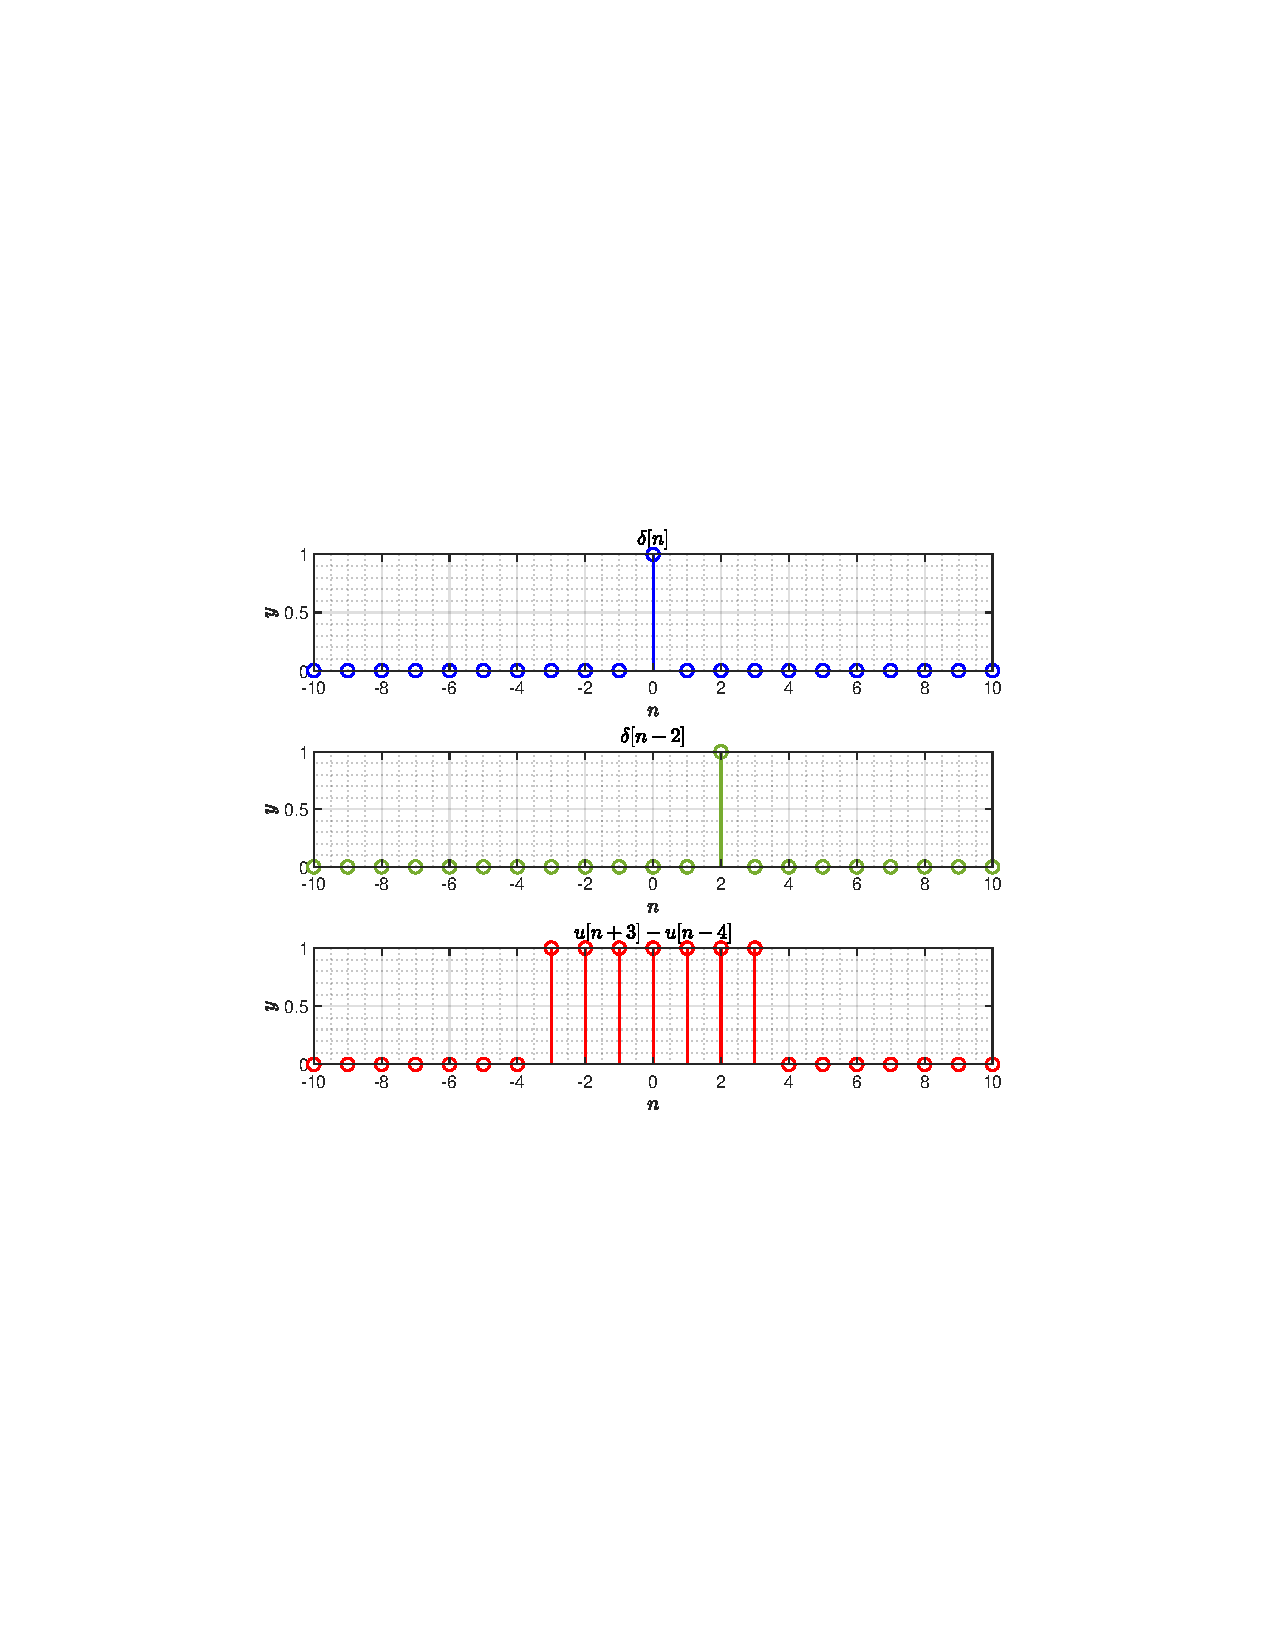
\includegraphics[width=\linewidth]{images/delta_dirac_function.pdf}
	\caption{تابع دلتا}
	\label{دلتا}
\end{figure}



\question 
تابعی به نام 
\lr{max}
بنویسید که دو عدد صحیح را به عنوان آرگومان ورودی گرفته ماکزیمم آنها را برگرداند.
\begin{parts}
\part[10] با دو \lr{return}
\part[10] با یک \lr{return}
\end{parts}

\question[20]
تابعی بازگشتی بنویسید که عددی را به عنوان آرگومان گرفته (مثلاً $x$) سه به توان آنرا ($3^x$) محاسبه و برگرداند. اگر بازگشتی ننویسید، بخشی از نمره را از دست خواهید داد.

\question[20]
تابعی بنویسید که دو عدد صحیح را به عنوان آرگومان پذیرفته، حاصل تقسیم اولی بر دومی را محاسبه و برگرداند. اگر عدد دوم صفر است پیام مناسبی چاپ کنید. اگر تابع ننویسید بخشی از نمره را از دست خواهید داد.

\question[30]
فرمول بسط سینوس به صورت زیر است:

\[ sin(x) = x - \frac{x^3}{3!} + \frac{x^5}{5!} - \frac{x^7}{7!} +  \cdots \]

برنامه‌ای برای محاسبه  مجموع ۲۰ جمله اول آن بنویسید.
در صورت تمایل می‌توانید تابعی برای محاسبه فاکتوریل بنویسید.

\end{questions}
\end{document}